\documentclass[tikz,border=7pt]{standalone}
% Shared visual language for the book's standalone vector figures.
% Keep this file compatible with the TeX Live version used by LyX.
\usepackage{amsmath,amssymb}
\usepackage{array,booktabs}
\usepackage{pgfplots}
\usepackage{pgfplotstable}
\usetikzlibrary{arrows.meta,calc,positioning}
\pgfplotsset{compat=1.17}

\definecolor{BookBlue}{HTML}{0072B2}
\definecolor{BookOrange}{HTML}{D55E00}
\definecolor{BookGreen}{HTML}{009E73}
\definecolor{BookGray}{HTML}{666666}
\definecolor{BookLightGray}{HTML}{D9D9D9}

\pgfplotsset{
  book axis/.style={
    axis line style={black!75,line width=0.55pt},
    tick style={black!75,line width=0.45pt},
    tick label style={font=\small},
    label style={font=\small},
    legend style={
      font=\small,
      draw=none,
      fill=none,
      cells={anchor=west},
    },
    grid style={BookLightGray,line width=0.35pt},
    major grid style={BookLightGray,line width=0.35pt},
  },
}

\begin{document}
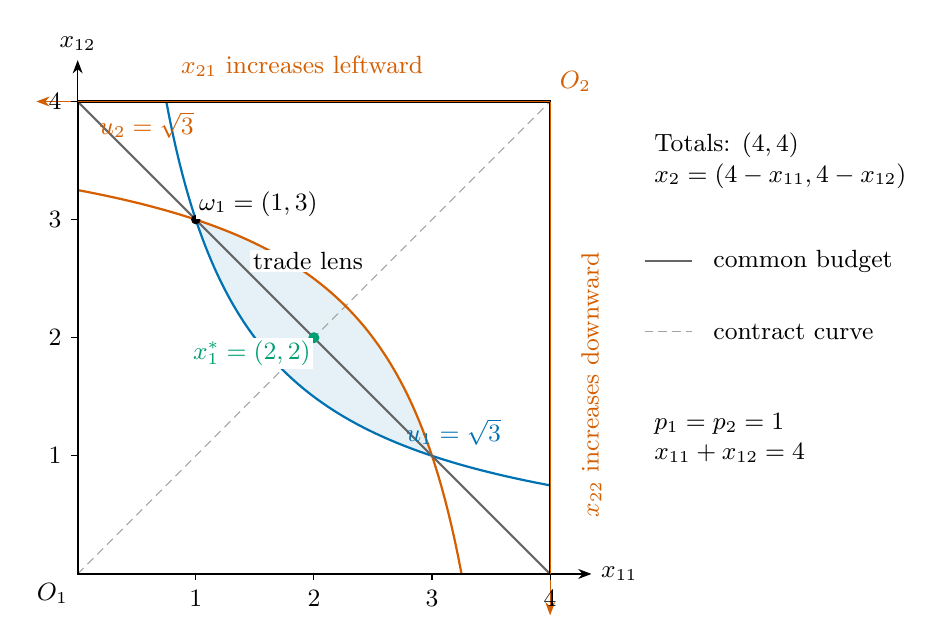
\begin{tikzpicture}[x=1.5cm,y=1.5cm,>=Stealth,font=\small]
  \fill[BookBlue!10] plot[domain=1:3,samples=100] (\x,{3/\x})
    -- plot[domain=3:1,samples=100] (\x,{4-3/(4-\x)}) -- cycle;
  \draw[BookGray!60,densely dashed] (0,0)--(4,4);
  \draw[BookBlue,thick,domain=.75:4,samples=120] plot (\x,{3/\x});
  \draw[BookOrange,thick,domain=0:3.25,samples=120] plot (\x,{4-3/(4-\x)});
  \draw[BookGray,thick] (0,4)--(4,0);
  \draw[thick] (0,0) rectangle (4,4);
  \draw[->] (0,0)--(4.35,0) node[right] {$x_{11}$};
  \draw[->] (0,0)--(0,4.35) node[above] {$x_{12}$};
  \draw[->,BookOrange] (4,4)--(-.35,4);
  \node[BookOrange] at (1.9,4.3) {$x_{21}$ increases leftward};
  \draw[->,BookOrange] (4,4)--(4,-.35);
  \node[BookOrange,rotate=90] at (4.35,1.6) {$x_{22}$ increases downward};
  \foreach \v in {1,2,3,4} {
    \draw (\v,0)--(\v,-.055) node[below] {$\v$};
    \draw (0,\v)--(-.055,\v) node[left] {$\v$};
  }
  \node[below left] at (0,0) {$O_1$};
  \node[above right,BookOrange] at (4,4) {$O_2$};
  \fill (1,3) circle(1.7pt) node[above right,fill=white,inner sep=1pt] {$\omega_1=(1,3)$};
  \fill[BookGreen] (2,2) circle(2pt) node[below left,fill=white,inner sep=1pt] {$x_1^*=(2,2)$};
  \node[BookBlue,anchor=west] at (2.7,1.2) {$u_1=\sqrt3$};
  \node[BookOrange,anchor=west] at (.1,3.8) {$u_2=\sqrt3$};
  \node[fill=white,inner sep=1pt] at (1.95,2.65) {trade lens};
  \node[anchor=west,align=left] at (4.8,3.5) {Totals: $(4,4)$\\$x_2=(4-x_{11},4-x_{12})$};
  \draw[BookGray] (4.8,2.65)--(5.2,2.65);
  \node[anchor=west] at (5.3,2.65) {common budget};
  \draw[BookGray!60,densely dashed] (4.8,2.05)--(5.2,2.05);
  \node[anchor=west] at (5.3,2.05) {contract curve};
  \node[anchor=west,align=left] at (4.8,1.15) {$p_1=p_2=1$\\$x_{11}+x_{12}=4$};
\end{tikzpicture}
\end{document}
